We tried to use the spectral clustering algorithm on other datasets, focusing on 3-dimensional clustering problems. Three datasets have been chosen to benchmark the algorithm: the \texttt{tetra}, \texttt{chainlink} and \texttt{atom} datasets. They were downloaded from this \href{https://github.com/deric/clustering-benchmark}{link}.

\begin{figure}[H]
    \centering
    \subfloat[1][\texttt{atom} dataset]{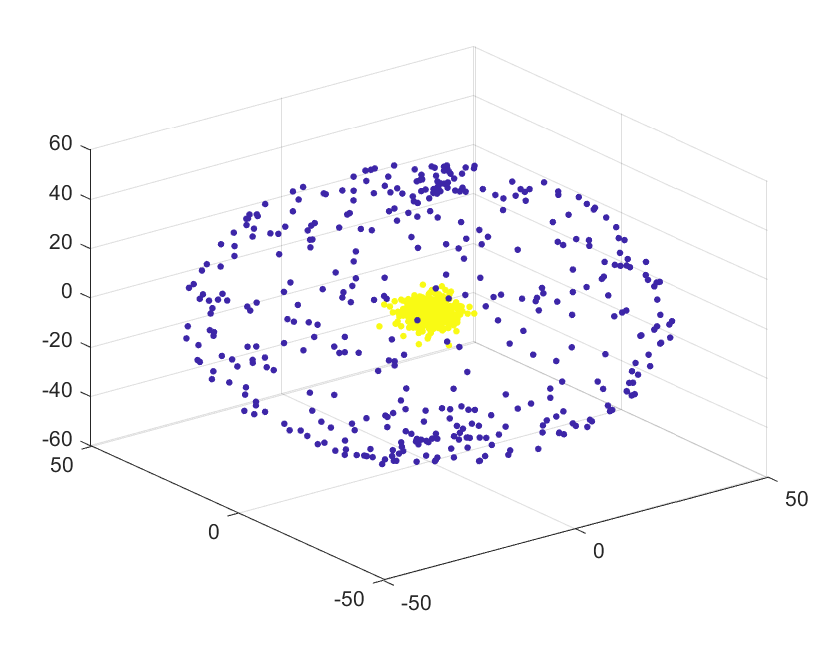
\includegraphics[scale = 0.37]{pictures/atom_scatterplot.pdf}}
    \subfloat[2][\texttt{tetra} dataset]{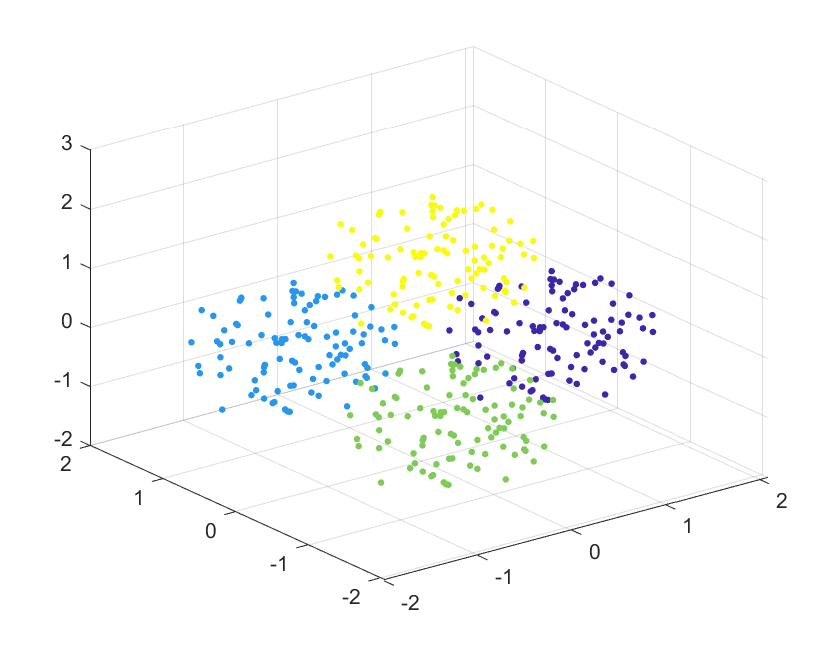
\includegraphics[scale = 0.37]{pictures/tetra_scatterplot.pdf}}
    \subfloat[3][\texttt{chainlink} dataset]{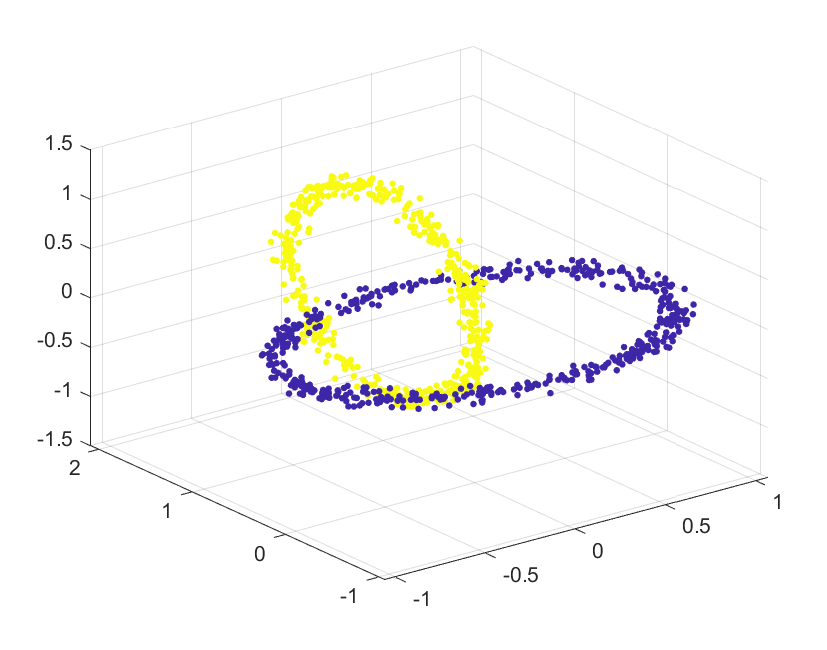
\includegraphics[scale = 0.37]{pictures/chainlink_scatterplot.pdf}}
    \caption{3D-scatterplots of the three datasets used for benchmarking}
    \label{scatterplot_3d}
      \end{figure}

\noindent Different values of \(K\) were used for these datasets. In particular, we experimented with values \(K \in \{5, 10, 20\}\). Plots of the adjacency graphs are shown for \(K=5\):

\begin{figure}[H]
    \centering
    \subfloat[1][\texttt{atom} dataset]{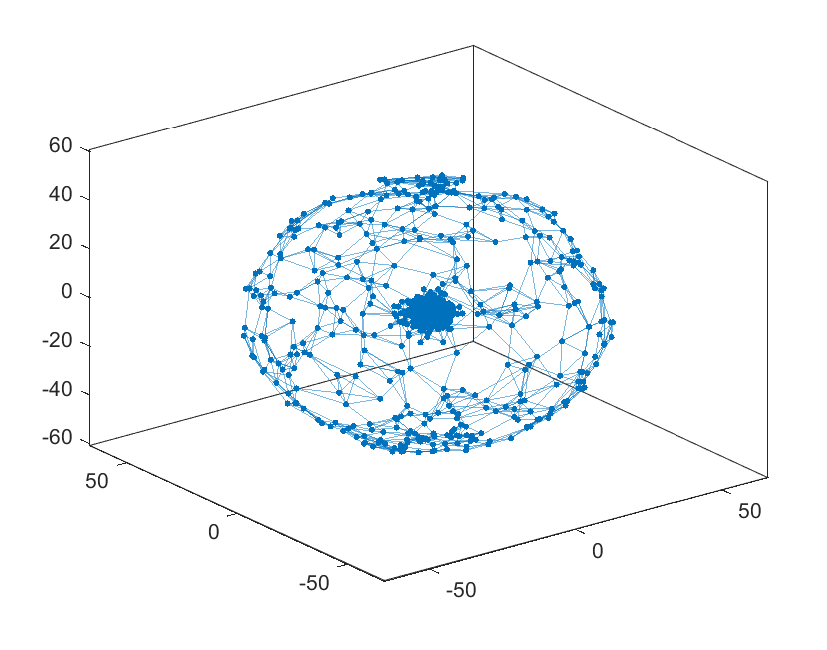
\includegraphics[scale = 0.37]{pictures/atom_KNN_K5.pdf}}
    \subfloat[2][\texttt{tetra} dataset]{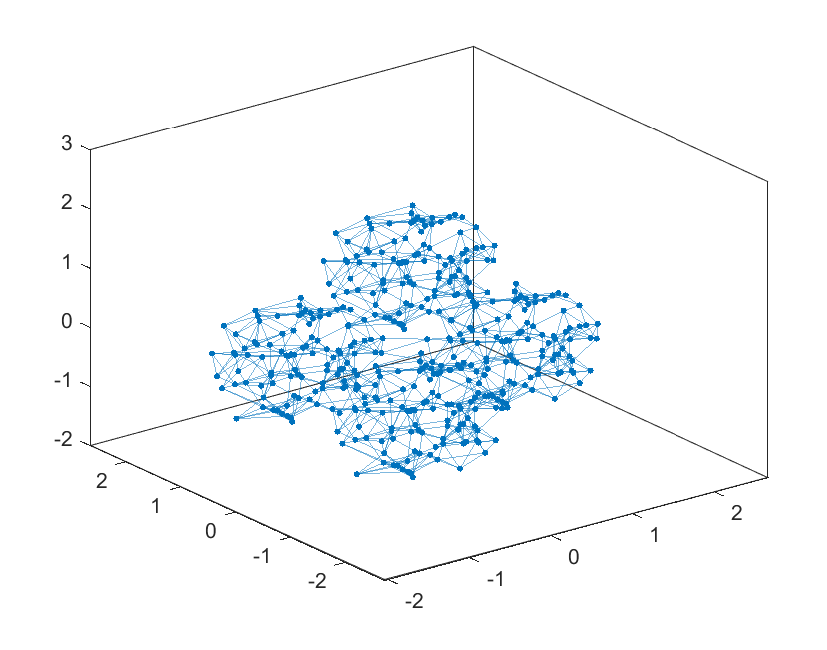
\includegraphics[scale = 0.37]{pictures/tetra_KNN_K5.pdf}}
    \subfloat[3][\texttt{chainlink} dataset]{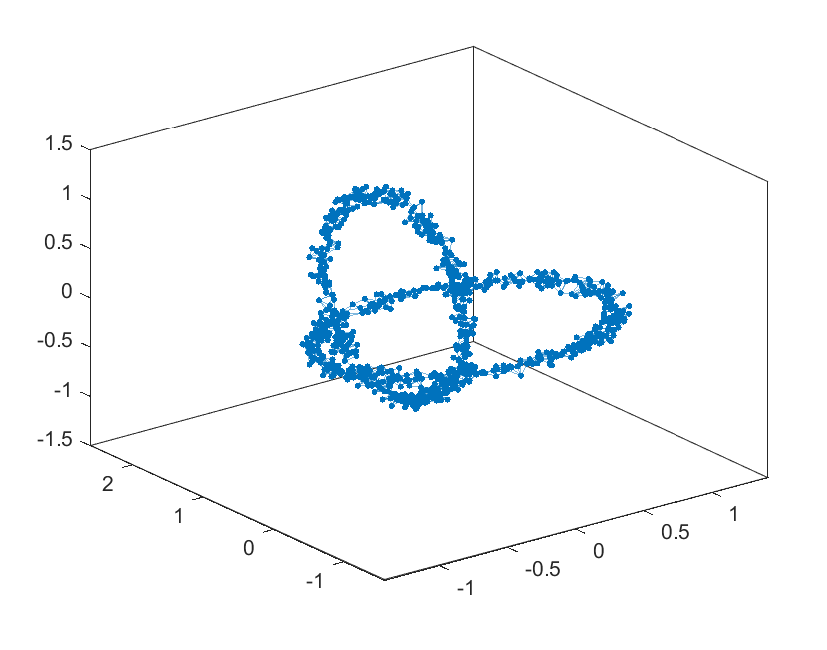
\includegraphics[scale = 0.37]{pictures/chainlink_KNN_K5.pdf}}
    \caption{Adjacency graph plot for the three datasets, computed with \(K=5\)}
    \label{adjacency_3d}
\end{figure}

\noindent For every dataset and every value of \(K\) we hence have an adjacency graph from which we can recover the relative Laplacian matrix \(L\). From a quick estimation of the conditioning number \(k\) we notice that each Laplacian matrix computed is \textbf{ill conditioned}, conditioning numbers span in fact from \(k \sim 10^{17}\) for the \texttt{tetra} dataset to \(k \sim 10^{61}\) \texttt{atom} dataset. 
The Laplacian matrix of the \texttt{atom} dataset is extremely ill conditioned and this will result in very inaccurate computation of its eigenvectors.
\\
As in \ref{sec3} we have chosen the number of cluster from evaluation of the eigenvalues of each Laplacian matrix \(L\) and used \(M=2\) for the \texttt{atom} dataset, \(M=4\) for \texttt{tetra} and \(M=2\) for \texttt{chainlink}.
\\
Performing the \textit{K-means} algorithm on the truncated eigenvector matrix as in \ref{sec4} produced the following results:

\begin{figure}[H]
    \centering
    \subfloat[1][\texttt{atom} dataset]{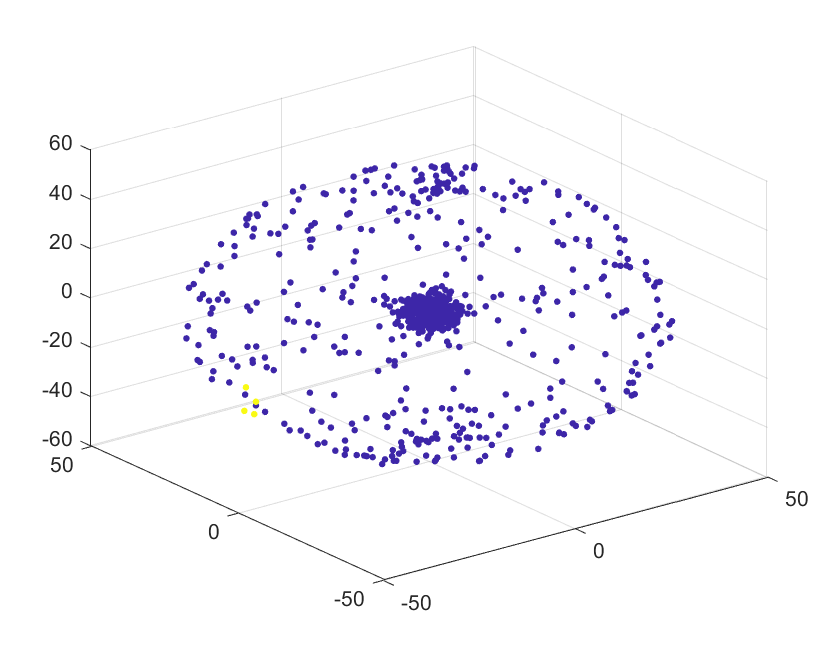
\includegraphics[scale = 0.37]{pictures/atom_SpectralClustering_K5.pdf}}
    \subfloat[2][\texttt{tetra} dataset]{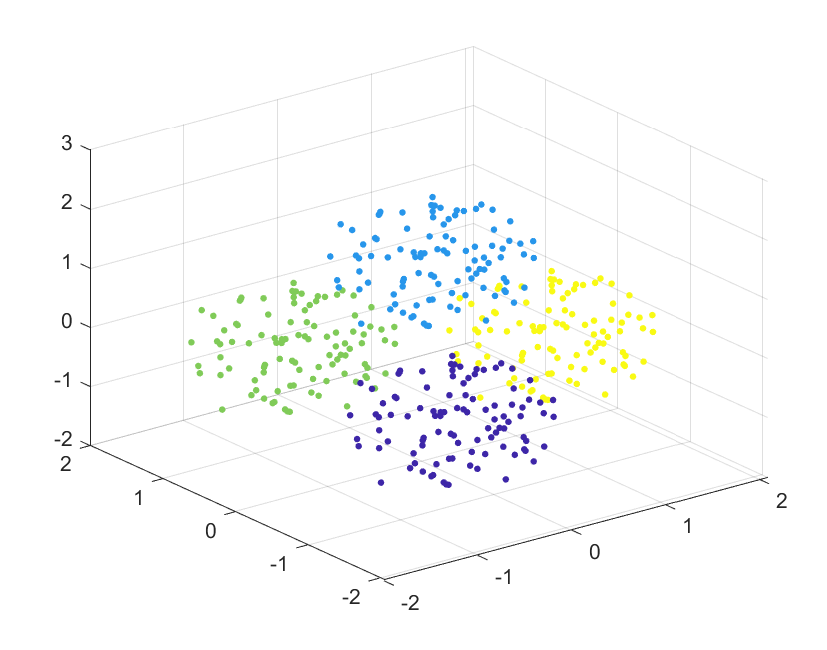
\includegraphics[scale = 0.37]{pictures/tetra_SpectralClustering_K10.pdf}}
    \subfloat[3][\texttt{chainlink} dataset]{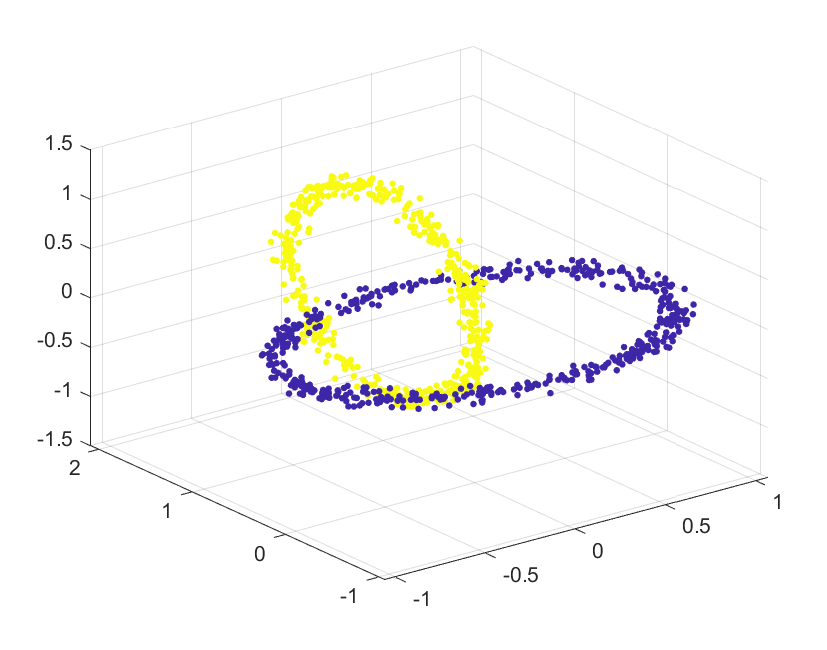
\includegraphics[scale = 0.37]{pictures/chainlink_SpectralClustering_K10.pdf}}
    \caption{Spectral clustering performed on three datasets, best results of \(K\) are shown}
    \label{SpectralClustering_3d}
\end{figure}

\noindent As it is clearly visible from figure \ref{SpectralClustering_3d} we can see that the Spectral Clustering Algorithm performs well on both \texttt{atom} and \texttt{chainlink} datasets while it is not able to correctly cluster points from the \texttt{atom} dataset. This is due to the fact that the computation of the eigenvalues for the Laplacian matrix \(L\) is very inaccurate due to its bad conditioning number.

